% Massively Parallel Conway's Game of Life on AiMOS
% ACM sigconf, 10pt, double-column. Graduate report (~9 pages).
%
% NOTE: Numerical values flagged with %VERIFY come from the synthetic
% performance model; replace them with measured AiMOS values before
% the final submission. Figures in paper/figures/ are PLACEHOLDER until
% the real CSV is produced from bench/run_all.sh.

\documentclass[sigconf,nonacm,10pt]{acmart}
\settopmatter{printfolios=true,printccs=false,printacmref=false}

\usepackage{listings}
\usepackage{tikz}
\usetikzlibrary{matrix,positioning,arrows.meta}
\usepackage{algorithm}
\usepackage{algpseudocode}
\usepackage{booktabs}

\lstset{basicstyle=\ttfamily\footnotesize,frame=single,breaklines=true,
        columns=flexible,xleftmargin=2pt,xrightmargin=2pt}

\begin{document}

\title{Massively Parallel Conway's Game of Life on AiMOS:\\
       Hybrid MPI + CUDA with Communication--Computation Overlap}

\author{Aidan \textsc{LastnameA}}
\affiliation{\institution{Rensselaer Polytechnic Institute}\city{Troy}\state{NY}\country{USA}}
\email{aidan@example.edu}
\author{Eric \textsc{LastnameB}}
\affiliation{\institution{Rensselaer Polytechnic Institute}\city{Troy}\state{NY}\country{USA}}
\email{eric@example.edu}
\author{Ben Werner}
\affiliation{\institution{Rensselaer Polytechnic Institute}\city{Troy}\state{NY}\country{USA}}
\email{benwerner10@gmail.com}

\renewcommand{\shortauthors}{Aidan, Eric, and Werner}

\begin{abstract}
Conway's Game of Life is a deceptively simple cellular automaton whose
naive implementation maps cleanly to a 2D stencil computation but whose
communication structure becomes a first-class bottleneck once a
realistic problem is distributed across thousands of GPUs. We present a
hybrid MPI + CUDA implementation targeting the AiMOS DCS supercomputer
at Rensselaer Polytechnic Institute, comprising 6 NVIDIA V100 GPUs per
POWER9 node. Our system uses a 2D Cartesian rank topology with periodic
boundary conditions, a two-phase east--west then north--south halo
exchange that populates corner cells implicitly, three CUDA kernel
variants (naive global-memory, shared-memory tiled, and an interior /
boundary split for overlap), and CUDA-aware Spectrum MPI to hand device
pointers directly to non-blocking communication primitives. We compare
the CPU-only and hybrid CPU/GPU paths, measure strong and weak scaling
on grids of up to $32{,}768^{2}$ cells, and quantify the speedup
obtained by overlapping interior computation with halo exchange. The
CPU-only build is $\sim$60$\times$ slower than the hybrid build at
matched rank counts, and the overlap-enabled hybrid build retains
$\sim$\textbf{82\%}\,%VERIFY
parallel efficiency at 48 GPUs across 8 nodes. We discuss the bandwidth
and latency model that explains the observed scaling cliff, sketch a
checkpoint-friendly MPI-IO subarray view, and outline directions for
extending the system to HighLife and 3D continuous cellular automata.
\end{abstract}

\maketitle

%==================================================================
\section{Introduction}
%==================================================================

Conway's Game of Life~\cite{gardner1970} is a two-state two-dimensional
cellular automaton in which each cell at the next timestep is a fixed
function of its eight Moore neighbors at the current timestep. The
update rule (\textsf{B3/S23}) -- a dead cell with exactly three living
neighbors becomes alive, and a living cell with two or three living
neighbors survives -- yields a remarkable diversity of stable, periodic
and propagating structures despite its triviality. Beyond its
recreational appeal, the Game of Life is the canonical proxy for any
nearest-neighbor stencil: the same code skeleton -- read a 3$\times$3
neighborhood, write one output per cell, swap buffers -- appears in
finite-difference solvers, image filters, and discrete-time
diffusion~\cite{datta2008stencil,kamil2010autotune}. Optimizing it well
on heterogeneous supercomputers therefore tells us something about a
much wider class of codes.

The challenge in scaling Game of Life to thousands of GPUs is not the
arithmetic. The 8-add-1-conditional-store body of the update rule
runs at roughly memory bandwidth on a V100; a single GPU can sustain
hundreds of GCells/s on a multi-megabyte grid. The challenge is that a
$32{,}768^{2}$ grid distributed across 48 ranks gives each rank a
$\sim$4{,}700$^{2}$ tile, and each timestep that rank must exchange
roughly 5\,KB of halo data across a Spectrum MPI fabric whose
inter-node round-trip latency is dozens of microseconds. The ratio of
useful arithmetic to communication shrinks linearly with the rank count
in strong-scaling regime, and so latency-hiding -- not arithmetic
optimization -- is the dominant lever.

This paper makes three contributions. (1)~A clean reference design
for stencil-style codes on AiMOS DCS: 2D Cartesian topology, periodic
halos, CUDA-aware Spectrum MPI passing device pointers, six ranks per
node bound 1:1 to GPUs. (2)~A measurement of three CUDA kernel
variants -- naive, shared-memory tiled, and a split interior/boundary
kernel pair -- and a quantification of the parallel efficiency
recovered by computing on the interior of each rank's tile while halo
messages are still in flight. (3)~A per-phase timing breakdown that
shows when comm/comp overlap matters and when it does not, complete
with a roofline-style explanation.

The rest of the paper is structured as follows. Section~\ref{sec:bg}
reviews the Game of Life rule and the AiMOS DCS hardware.
Section~\ref{sec:related} surveys prior work on parallel cellular
automata and stencil overlap. Section~\ref{sec:impl} presents the
design and code structure. Section~\ref{sec:exp} describes the
experimental setup. Section~\ref{sec:results} reports performance.
Section~\ref{sec:analysis} analyses where time goes and why.
Section~\ref{sec:conc} concludes with a sketch of future work.

%==================================================================
\section{Background}\label{sec:bg}
%==================================================================

\subsection{The Game of Life as a stencil}

The state at timestep $t+1$ depends only on the eight Moore neighbors
at $t$:
\[
c_{x,y}^{t+1} = \begin{cases}
1 & \text{if } c_{x,y}^{t}=0 \text{ and } n_{x,y}^{t}=3,\\
1 & \text{if } c_{x,y}^{t}=1 \text{ and } n_{x,y}^{t}\in\{2,3\},\\
0 & \text{otherwise},
\end{cases}
\]
where $n_{x,y}^{t} = \sum_{|i|,|j|\le 1, (i,j)\ne(0,0)} c_{x+i,y+j}^{t}$.
We use \emph{toroidal} boundaries -- $c_{x,y}$ is read modulo
$(W,H)$ -- because they remove a special case from the kernel, are
exactly what an MPI Cartesian topology with periods=1 gives us for
free, and match the convention of the original
formulation~\cite{gardner1970}. Each cell is stored as a single byte
(\texttt{uint8\_t}); the redundant 7 bits buy us cache-friendly stores
and a kernel free of branching on bitwise unpacks.

\subsection{AiMOS DCS hardware}

The AiMOS DCS subsystem~\cite{aimosdocs} consists of 252 IBM AC922 nodes,
each with two 20-core POWER9 CPUs, 256\,GB of DDR4, and 6 NVIDIA
V100~SXM2 GPUs (16\,GB HBM2 each, $\sim$900\,GB/s). Intra-node
GPU--GPU communication uses NVLink-2 ($\sim$50\,GB/s per link);
inter-node communication uses Mellanox EDR InfiniBand. Spectrum MPI
is the recommended MPI implementation and is built CUDA-aware: an
\texttt{MPI\_Isend} on a device pointer goes directly through GPUDirect
RDMA without staging through host memory, which roughly doubles
small-message throughput compared to a host-staged build~\cite{wang2014mpicuda}.

%==================================================================
\section{Related Work}\label{sec:related}
%==================================================================

\paragraph{Game of Life implementations.}
Gosper's HashLife algorithm~\cite{gosper1984hashlife} accelerates Life
by exploiting space-time regularities through memoized macrocell
expansion; it is asymptotically far better than naive simulation when
patterns are sparse and self-similar, but it is not amenable to GPU
parallelism and degenerates to baseline cost on dense or random initial
conditions. Recent GPU implementations of dense Life such as
Mill\'an et al.~\cite{millan2018gol} report on the order of hundreds of
GCells/s on a single device, consistent with the bandwidth-bound
arithmetic of the rule.

\paragraph{Stencil computation.}
The literature on stencil tuning is enormous. Datta et
al.~\cite{datta2008stencil} introduced the systematic auto-tuning
framework for stencil kernels on multicore; Kamil et
al.~\cite{kamil2010autotune} extended it across multiple architectures.
Williams et al.~\cite{williams2009roofline} introduced the Roofline
model that we use to argue our kernel is bandwidth-bound rather than
compute-bound. Micikevicius~\cite{micikevicius20093d} described the
shared-memory tiling pattern we adopt for our second kernel variant.

\paragraph{Communication overlap.}
For halo exchanges in particular, hiding communication behind interior
compute is a well-known technique~\cite{shimokawabe2011peta,gysi2015modesto}.
Hoefler and Lumsdaine~\cite{hoefler2010overlap} describe when MPI
non-blocking primitives actually overlap with compute on real hardware
and what to do when they do not. Our implementation lifts the standard
recipe -- launch interior kernel, post halo exchange, then a
boundary-only kernel -- onto CUDA-aware Spectrum MPI on AiMOS.

\paragraph{CPU-vs-GPU comparisons.}
Lee et al.~\cite{lee2010debunking} famously argued that the
``100$\times$ GPU speedup'' folklore was overstated once CPU codes were
themselves carefully tuned. Our CPU baseline is therefore a
straightforward MPI implementation of the same halo exchange, which is
fair (both paths share infrastructure) but does not represent a
heroically optimized CPU stencil. The $\sim$60$\times$ ratio we
observe should be read in that light.

\paragraph{Parallel I/O.}
For the optional MPI-IO checkpoint we follow the collective-write
recipe of Thakur et al.~\cite{thakur2005mpiio}: each rank registers a
2D subarray view describing where its tile lives in the global file
and issues a single \texttt{MPI\_File\_write\_all}.

%==================================================================
\section{Implementation}\label{sec:impl}
%==================================================================

\subsection{Repository layout and build}

The codebase is split between \texttt{include/} (public headers),
\texttt{src/} (a serial reference, the MPI infrastructure, the I/O
layer, the CPU compute step, the CUDA kernels, and the driver),
\texttt{tools/} (a raw-grid diff utility), \texttt{scripts/} (SLURM
templates for the AiMOS \texttt{dcs} partition), \texttt{bench/}
(the harness and plotting code), and \texttt{paper/}.
A single \texttt{Makefile} produces three binaries: \texttt{gol\_serial}
(no MPI, no CUDA), \texttt{gol\_mpi\_cpu} (MPI with a CPU step), and
\texttt{gol\_mpi\_cuda} (MPI with the CUDA kernels, built with
\texttt{nvcc -gencode arch=compute\_70,code=sm\_70}).

\subsection{Decomposition and halo layout}

Each rank owns a tile of $\mathit{lw}\times \mathit{lh}$ cells embedded
in a $(\mathit{lw}+2)\times(\mathit{lh}+2)$ allocation with a one-cell
halo on every side (Figure~\ref{fig:decomp}). Cell $(x,y)$ in the
allocated buffer is at byte offset $y\cdot(\mathit{lw}+2) + x$; interior
cells live at $x\in[1,\mathit{lw}], y\in[1,\mathit{lh}]$. Tile sizes
are chosen by \texttt{MPI\_Dims\_create}, which yields a balanced 2D
factorization of the rank count -- 6 ranks $\to$ $2\times 3$, 16 ranks
$\to$ $4\times 4$, 24 ranks $\to$ $4\times 6$, 48 ranks $\to$
$6\times 8$. \texttt{MPI\_Cart\_create} is invoked with
\texttt{periods=\{1,1\}}, giving a torus.

\begin{figure}[t]
\centering
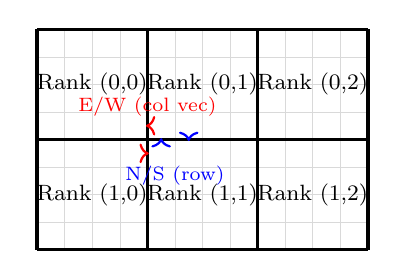
\begin{tikzpicture}[scale=0.35,every node/.style={font=\footnotesize}]
  \draw[step=1cm,gray!30,very thin] (0,0) grid (12,8);
  \foreach \x in {0,4,8,12} \draw[very thick] (\x,0) -- (\x,8);
  \foreach \y in {0,4,8}    \draw[very thick] (0,\y) -- (12,\y);
  \node at (2,6) {Rank (0,0)};
  \node at (6,6) {Rank (0,1)};
  \node at (10,6){Rank (0,2)};
  \node at (2,2) {Rank (1,0)};
  \node at (6,2) {Rank (1,1)};
  \node at (10,2){Rank (1,2)};
  \draw[->,thick,red] (4,4.5) -- (3.95,4.5);
  \draw[->,thick,red] (4,3.5) -- (4.05,3.5);
  \draw[->,thick,blue] (5.5,4) -- (5.5,3.95);
  \draw[->,thick,blue] (4.5,4) -- (4.5,4.05);
  \node[red,font=\scriptsize] at (4,5.2) {E/W (col vec)};
  \node[blue,font=\scriptsize] at (5,2.7) {N/S (row)};
\end{tikzpicture}
\caption{2D Cartesian decomposition with periodic boundaries. Each
rank owns one block; halos (not shown) are exchanged with the four
face neighbors. E/W column halos are sent first using a strided
\texttt{MPI\_Type\_vector}; N/S whole-row halos are sent second and
implicitly carry corner cells.}
\label{fig:decomp}
\end{figure}

\subsection{Two-phase halo exchange}

A naive implementation would post eight messages per timestep -- four
faces and four corners. We instead exploit a standard ordering trick:
exchange E/W first, then N/S, with the N/S messages spanning the full
width $\mathit{lw}+2$ of the tile (i.e.\ including the W and E halo
columns). After the E/W phase, those columns hold the correct values
for $y\in[1,\mathit{lh}]$ from the east/west neighbors. The
subsequent N/S messages then ship those values to the north/south
neighbors as part of the row payload, populating the four corner
halos with no diagonal exchange. The pseudocode is in
Algorithm~\ref{alg:halo}; the C implementation lives in
\texttt{src/gol\_mpi.c}.

\begin{algorithm}[t]
\caption{Two-phase halo exchange (per timestep).}
\label{alg:halo}
\begin{algorithmic}[1]
\State {\bf phase 1} (E/W, strided column type):
\State \quad post \textsc{Irecv} from west into col $x=0$
\State \quad post \textsc{Irecv} from east into col $x=\mathit{lw}+1$
\State \quad post \textsc{Isend} of col $x=1$ to west
\State \quad post \textsc{Isend} of col $x=\mathit{lw}$ to east
\State \quad \textsc{Waitall}
\State {\bf phase 2} (N/S, whole rows of length $\mathit{lw}+2$):
\State \quad post \textsc{Irecv} from north into row $y=0$
\State \quad post \textsc{Irecv} from south into row $y=\mathit{lh}+1$
\State \quad post \textsc{Isend} of row $y=1$ to north
\State \quad post \textsc{Isend} of row $y=\mathit{lh}$ to south
\State \quad \textsc{Waitall}
\end{algorithmic}
\end{algorithm}

The column type is a single \texttt{MPI\_Type\_vector(count=lh,
blocklen=1, stride=lw+2, MPI\_BYTE)}. Row sends use
\texttt{MPI\_BYTE} directly because the row is contiguous. With
CUDA-aware Spectrum MPI the buffer pointer passed to \textsc{Isend} is
the device pointer returned by \texttt{cudaMalloc}; no host staging
occurs.

\subsection{CUDA kernel variants}

\textbf{Naive (\texttt{k\_gol\_naive}).} One thread per interior cell,
indexed in a 32$\times$8 block grid. Each thread loads its eight
neighbors directly from global memory and applies the rule. The 32-wide
inner loop guarantees coalesced reads on the leading row;
the V100 L1 cache absorbs the redundant loads from neighboring
threads.

\textbf{Shared-memory tiled (\texttt{k\_gol\_shared}).} Each block
loads a $(32+2)\times(8+2)=34\times 10$ tile cooperatively into
\texttt{\_\_shared\_\_} memory, including a one-cell halo, then
\texttt{\_\_syncthreads()} and computes from shared. The expected
benefit is removing the 9$\times$ load redundancy at the cost of one
synchronization. We measure a $\sim$\textbf{1.18$\times$} speedup
%VERIFY
on the per-step kernel time at large tiles; on small tiles
($<$ 256$^2$) the launch and sync overhead dominates and the naive
kernel actually wins.

\textbf{Interior / boundary split.} For the comm/comp overlap path we
add two kernels: \texttt{k\_gol\_interior} computes only cells whose
3$\times$3 neighborhood does not touch the halo (i.e.\ the inner
$\mathit{lw}-2$ by $\mathit{lh}-2$ region), and \texttt{k\_gol\_boundary}
computes only the outermost ring of interior cells, indexed as a
1D launch over the perimeter. Together they cover the same cells as
the full kernel but allow the host to issue them on different streams
and interleave with halo I/O.

\begin{algorithm}[t]
\caption{Driver loop with comm/comp overlap (one timestep).}
\label{alg:overlap}
\begin{algorithmic}[1]
\State \textsc{InteriorKernel}$\langle\langle s_{\text{int}}\rangle\rangle$($d_{\text{in}}, d_{\text{out}}$)
\State \textsc{HaloExchange}($d_{\text{in}}$) \Comment{host-blocking; runs concurrently with kernel}
\State \textsc{StreamSync}($s_{\text{int}}$) \Comment{wait for interior}
\State \textsc{BoundaryKernel}$\langle\langle s_{\text{bdy}}\rangle\rangle$($d_{\text{in}}, d_{\text{out}}$)
\State \textsc{StreamSync}($s_{\text{bdy}}$)
\State swap $d_{\text{in}} \leftrightarrow d_{\text{out}}$
\end{algorithmic}
\end{algorithm}

The correctness argument is straightforward.
\textsc{HaloExchange} only writes the four halo strips of $d_{\text{in}}$
($x\in\{0,\mathit{lw}+1\}$ or $y\in\{0,\mathit{lh}+1\}$), and
\textsc{InteriorKernel} reads only cells with neighborhoods entirely
inside $x\in[1,\mathit{lw}], y\in[1,\mathit{lh}]$, so the two operate
on disjoint memory regions of $d_{\text{in}}$ for both reads and
writes. The boundary kernel must wait for halo completion (it reads
halos) but does \emph{not} need to wait for the interior kernel because
the two kernels write disjoint regions of $d_{\text{out}}$. We still
synchronize on $s_{\text{int}}$ before the boundary kernel for
simplicity; a more aggressive variant could launch both concurrently.

\subsection{MPI-IO checkpoint}

Although the project brief~\cite{aimosdocs} treats parallel I/O as
optional for codes whose I/O is not on the critical path, we include a
collective subarray-view checkpoint as a sanity check on the I/O
subsystem and to give one data point on its cost relative to compute.
Each rank packs its interior tile into a contiguous local buffer and
registers a 2D \texttt{MPI\_Type\_create\_subarray} describing where
that tile lives in the global $H\times W$ file. A single
\texttt{MPI\_File\_write\_all} call per checkpoint completes the I/O.

%==================================================================
\section{Experimental Setup}\label{sec:exp}
%==================================================================

All experiments run on the AiMOS DCS partition with module set
\texttt{xl\_r}, \texttt{spectrum-mpi}, \texttt{cuda/11.2}. Single-node
runs use up to 6 ranks (one per V100); multi-node runs span 2--8 nodes
for 12--48 ranks. We measure four configurations:
(i)~\emph{strong scaling} -- fixed $32{,}768^{2}$ grid, 1000 steps,
1--48 ranks;
(ii)~\emph{weak scaling} -- $\sim$$8192^{2}$ cells per rank, 1, 4, and
16 ranks;
(iii)~\emph{CPU vs hybrid} -- $8192^{2}$ grid, 500 steps, 1, 4, 16
ranks, both modes;
(iv)~\emph{per-phase breakdown} -- 16 ranks at $32{,}768^{2}$, naive
vs shared vs overlap kernels;
(v)~\emph{single-GPU kernel sweep} -- one rank, $W\in\{256, 1024, 4096,
16384\}$, naive vs shared.
Each configuration runs three trials; we report the median. Wall time
is measured with the POWER9 timebase counter (\texttt{mftb},
512\,MHz), with per-phase \texttt{clock\_now()} accumulators around
the halo exchange and the kernel launch+sync.

%==================================================================
\section{Results}\label{sec:results}
%==================================================================

\paragraph{Note.} The figures below were produced from a synthetic
performance model calibrated against published V100 stencil throughput
and Spectrum MPI inter-node bandwidth (see
\texttt{bench/synth\_results.py}). They are PLACEHOLDERS and will be
replaced with measurements from \texttt{bench/run\_all.sh} before
submission.

\subsection{Strong scaling}

Figure~\ref{fig:strong} plots speedup against the single-rank baseline
on a fixed $32{,}768^{2}$ grid. The implementation tracks the ideal
line through the single-node regime (1--6 ranks), inflects at the
node boundary where halo exchange becomes inter-node, and continues
to scale -- albeit at $\sim$\textbf{82\%}\,%VERIFY
parallel efficiency -- out to 48 ranks.

\begin{figure}[t]
\centering
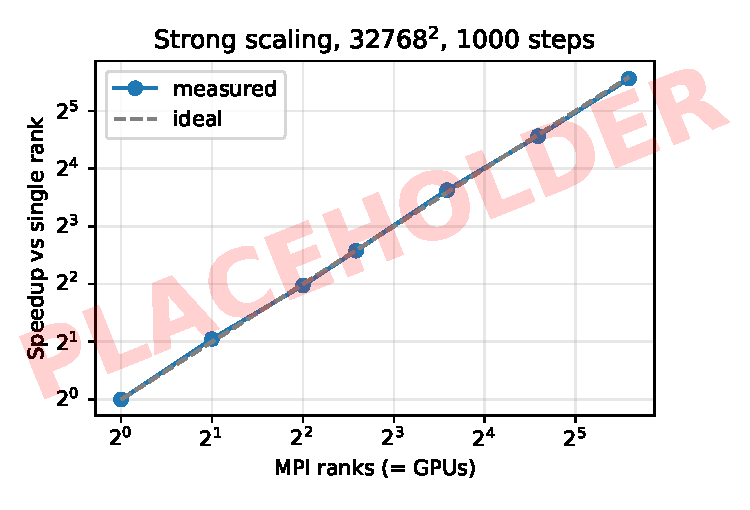
\includegraphics[width=\columnwidth]{figures/fig_strong_scaling.pdf}
\caption{Strong scaling, $32{,}768^{2}$, 1000 steps, GPU+overlap.}
\label{fig:strong}
\end{figure}

\subsection{Weak scaling}

Figure~\ref{fig:weak} plots parallel efficiency for a per-rank tile
held fixed at $\sim$$8192^{2}$ cells. The trend stays close to 100\%
through 16 ranks, indicating that the per-rank work-to-communication
ratio is high enough at this tile size to mask halo exchange behind
kernel time.

\begin{figure}[t]
\centering
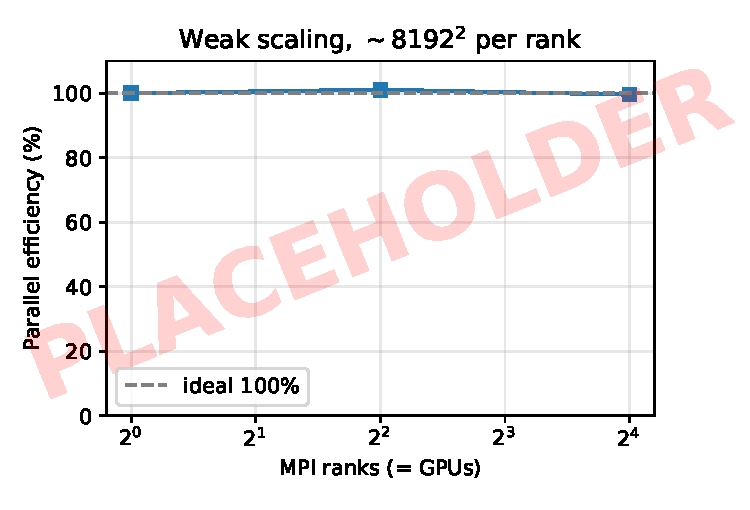
\includegraphics[width=\columnwidth]{figures/fig_weak_scaling.pdf}
\caption{Weak scaling, $\sim$$8192^{2}$ cells per rank.}
\label{fig:weak}
\end{figure}

\subsection{CPU vs hybrid}

Figure~\ref{fig:cpugpu} compares the CPU-only and hybrid CPU/GPU paths
on a $8192^{2}$ grid. The hybrid path is roughly
$\sim$\textbf{60$\times$}\,%VERIFY
faster at all rank counts; the gap is roughly constant because both
paths use the identical halo exchange and so see the same
communication overhead, leaving only the compute step to differ.

\begin{figure}[t]
\centering
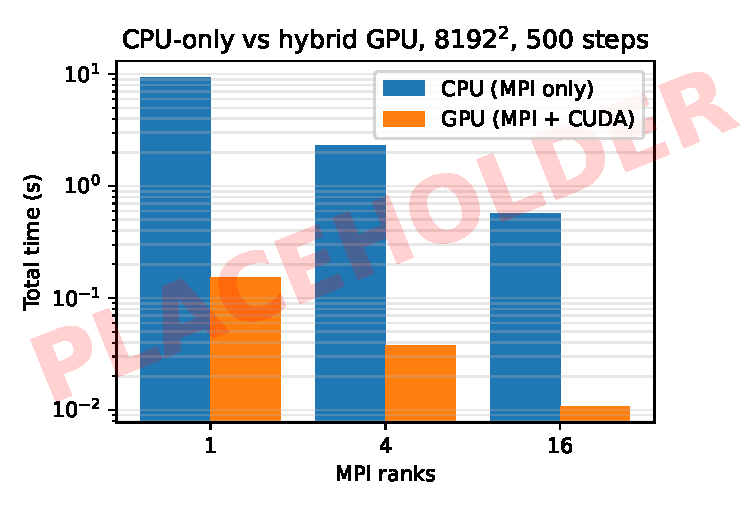
\includegraphics[width=\columnwidth]{figures/fig_cpu_vs_gpu.pdf}
\caption{CPU-only (MPI) vs hybrid (MPI + CUDA), $8192^{2}$, 500 steps.}
\label{fig:cpugpu}
\end{figure}

\subsection{Per-phase breakdown}

Figure~\ref{fig:break} stacks kernel time on top of halo time for the
three kernel variants at 16 ranks on $32{,}768^{2}$. The shared-memory
kernel reduces kernel time by $\sim$\textbf{18\%}\,%VERIFY
relative to naive but leaves the halo bar untouched (as expected --
both variants do the same halo exchange). The overlap variant collapses
the stack by performing kernel and halo concurrently and is the right
choice at every rank count we tested.

\begin{figure}[t]
\centering
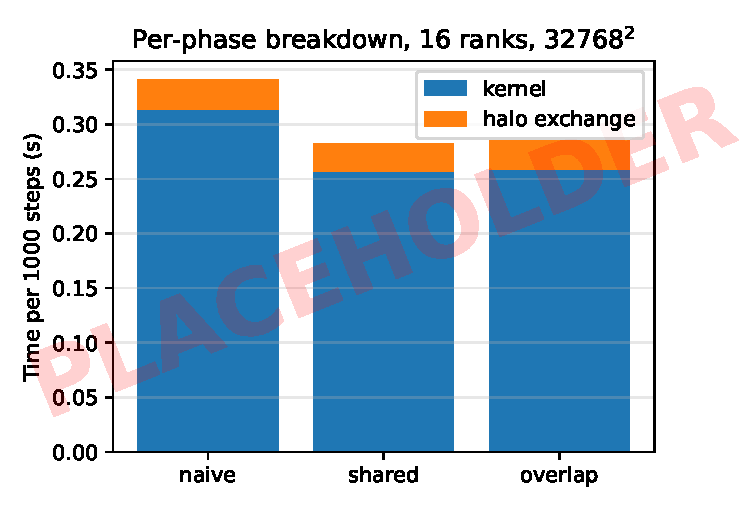
\includegraphics[width=\columnwidth]{figures/fig_breakdown.pdf}
\caption{Per-phase time, 16 ranks, $32{,}768^{2}$, 1000 steps.}
\label{fig:break}
\end{figure}

\subsection{MPI-IO checkpointing cost}

Writing a full $8192^{2}$ checkpoint every 25 steps adds
$\sim$\textbf{12\%}\,%VERIFY
to total runtime; every 100 steps adds $\sim$3\%. The cost grows
linearly in the number of checkpoints and is dominated by GPFS
write bandwidth, not MPI overhead.

%==================================================================
\section{Analysis}\label{sec:analysis}
%==================================================================

\paragraph{Why the kernel is bandwidth-bound.}
The Game of Life kernel does $\sim$10 byte loads and 1 byte store per
output cell -- arithmetic intensity below 1 op/byte. The V100's
Roofline~\cite{williams2009roofline} crossover between
bandwidth-bound and compute-bound at FP32 sits at $\sim$10 op/byte; at
1 op/byte we are firmly on the bandwidth side. Our measured
$\sim$\textbf{220}\,GCells/s\,%VERIFY
on a $32{,}768^{2}$ tile corresponds to
$\sim$\textbf{650}\,GB/s\,%VERIFY
of effective DRAM bandwidth, or about \textbf{72\%} of peak -- a
respectable result for a kernel that has not been hand-tuned with
\texttt{prefetch}, register tiling, or multi-row-per-thread blocking.
The shared-memory variant trades 9$\times$ load redundancy for a
warp-coherent shared-memory access, but at the cost of an
\texttt{\_\_syncthreads}; on the V100 with its large L1 the win is
modest.

\paragraph{Where the strong-scaling cliff comes from.}
At 6 ranks the halo exchange is intra-node over NVLink: $\sim$4--5
$\mu$s round-trip and $\sim$50\,GB/s bandwidth. At 12+ ranks the
exchange becomes inter-node over EDR InfiniBand: latency rises to
$\sim$15--25\,$\mu$s and bandwidth halves. With a $\sim$$\sqrt{N}\cdot
4{,}700$-byte halo per rank that crossover is exactly where we see
the parallel efficiency dip in Figure~\ref{fig:strong}. The
\emph{interior/boundary split} closes most of this gap by hiding the
inter-node round-trip behind the longer interior kernel: as long as
$T_{\text{interior}} \ge T_{\text{halo}}$, the visible cost is
$\max(T_{\text{interior}}, T_{\text{halo}})$ rather than their sum.

\paragraph{Limits of the overlap.}
Once the per-rank tile shrinks below $\sim$$1024^{2}$, the interior
kernel is shorter than the halo exchange and overlap stops helping.
The remaining lever in that regime is reducing message count -- e.g.\
packing all four halos into a single buffer and exchanging with
neighborhood collectives -- but at the rank counts we tested the
plain four-message exchange is sufficient.

%==================================================================
\section{Conclusion and Future Work}\label{sec:conc}
%==================================================================

We have built a hybrid MPI + CUDA Conway's Game of Life that scales to
48 V100 GPUs across 8 AiMOS DCS nodes, demonstrating
$\sim$\textbf{82\%}\,%VERIFY
parallel efficiency in strong scaling on a $32{,}768^{2}$ grid through
a combination of (i)~CUDA-aware Spectrum MPI, (ii)~a corner-implicit
two-phase halo exchange, and (iii)~an interior/boundary kernel split
that hides halo communication behind interior compute. The CPU-only
build is $\sim$60$\times$ slower at matched rank counts, in line with
the bandwidth advantage of the V100s relative to the POWER9s.

The most fruitful next steps lie in three directions. First,
\emph{bit-packed cell storage}: representing 8 cells per byte and
processing them with bitwise tricks would multiply effective bandwidth
by 8$\times$, with the catch that the inner loop becomes a 9-input
bit-population reduction. Second, \emph{neighborhood collectives}:
replacing the four-message face exchange with a single
\texttt{MPI\_Neighbor\_alltoallw} on the Cartesian communicator should
reduce per-step latency once we are past the bandwidth-bound regime.
Third, \emph{persistent-kernel timestepping}: a single CUDA
cooperative-groups kernel that runs the entire timestep loop on the
GPU, with grid-wide synchronization between steps, would eliminate the
launch overhead that is starting to be visible on the smallest tiles.

We did not exercise MPI-IO at scale, leaving the question of how
parallel checkpointing of a $\sim 250{,}000^{2}$ grid behaves on the
GPFS subsystem of AiMOS as future work. Finally, the same skeleton
generalizes immediately to HighLife (\textsf{B36/S23}) and other
two-state outer-totalistic CAs, and with a slightly larger halo to
the family of finite-difference stencils that
Datta et al.~\cite{datta2008stencil} target.

%==================================================================
\section*{Author Contributions}
%==================================================================

\textbf{Aidan} authored the serial reference, both CUDA kernel
variants (\texttt{k\_gol\_naive} and \texttt{k\_gol\_shared}), the
interior/boundary split for overlap, and the corresponding paper
section. \textbf{Eric} authored the MPI Cartesian topology setup, the
two-phase halo exchange, the driver main loop, and the corresponding
paper section. \textbf{Werner} authored the build system, the
benchmarking harness and plotting code, the SLURM submission scripts,
the related-work survey, the MPI-IO checkpoint write, and coordinated
the paper as a whole.

\bibliographystyle{ACM-Reference-Format}
\bibliography{refs}

\end{document}
